\clearpage
\subsection{MSVC + \olly}
\myindex{\olly}

Let's try this example in \olly.
Let's load it and keep pressing F8 (\stepover) until we reach our executable file instead of \TT{ntdll.dll}.
Scroll up until \main appears.

Click on the first instruction (\TT{PUSH EBP}), press F2 (\IT{set a breakpoint}), then F9 (\IT{Run}).
The breakpoint will be triggered when \main begins.

Let's trace to the point where the address of the variable $x$ is calculated:

\begin{figure}[H]
\centering
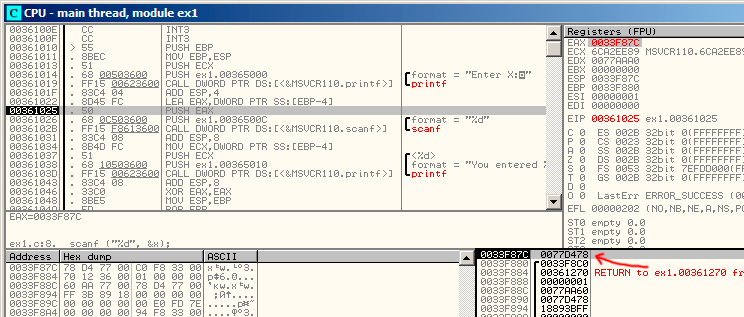
\includegraphics[scale=\FigScale]{patterns/04_scanf/1_simple/ex1_olly_1.png}
\caption{\olly: The address of the local variable is calculated}
\label{fig:scanf_ex1_olly_1}
\end{figure}

Right-click the \EAX in the registers window and then select \q{Follow in stack}.

This address will appear in the stack window.
The red arrow has been added, pointing to the variable in the local stack.
At that moment this location contains some garbage (\TT{0x6E494714}).
Now with the help of \PUSH instruction the address of this stack element is going to be stored to the same stack on the next position.
Let's trace with F8 until the \scanf execution completes.
During the \scanf execution, we input, for example, 123, in the console window:

\begin{figure}[H]
\centering
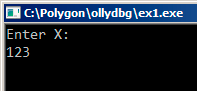
\includegraphics[scale=\NormalScale]{patterns/04_scanf/1_simple/ex1_olly_2.png}
\caption{User input in the console window}
\label{fig:scanf_ex1_olly_2}
\end{figure}

\clearpage
\scanf completed its execution already:

\begin{figure}[H]
\centering
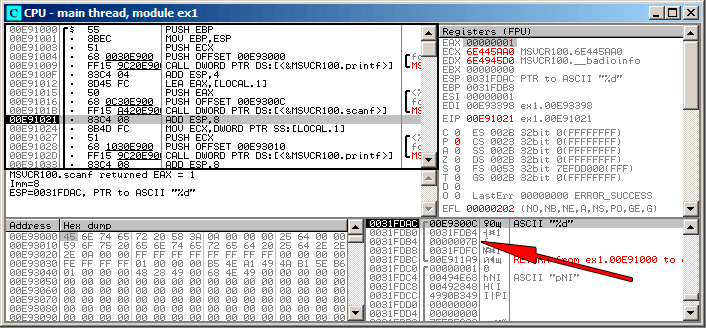
\includegraphics[scale=\FigScale]{patterns/04_scanf/1_simple/ex1_olly_3.png}
\caption{\olly: \scanf executed}
\label{fig:scanf_ex1_olly_3}
\end{figure}

\scanf returns 1 in \EAX, which implies that it has read successfully one value.
If we look again at the stack element corresponding to the local variable it now contains \TT{0x7B} (123).

\clearpage

Later this value is copied from the stack to the \ECX register and passed to \printf:

\begin{figure}[H]
\centering
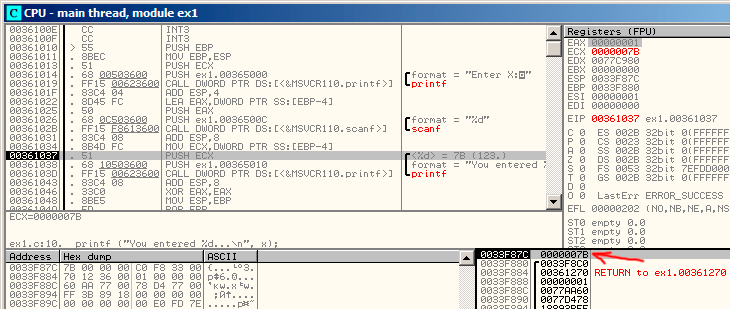
\includegraphics[scale=\FigScale]{patterns/04_scanf/1_simple/ex1_olly_4.png}
\caption{\olly: preparing the value for passing to \printf}
\label{fig:scanf_ex1_olly_4}
\end{figure}
